%**************************************************************
% Capitolo 3 - COSA-COME - Il prodotto dello stage
%**************************************************************
\chapter{Il prodotto\label{cap:ilprodotto}}
\section{Acquisizione delle conoscenze settoriali}
	 \subsection{Codifica video}
	 %TODO: Definizione di codifica video
	 %TODO: Definizione di codec

	 \subsection{Formati video comunemente usati}
			\subsubsection{M-JPEG}
			Motion JPEG	è un codec video che comprime ogni frame del video originale in una immagine in formato JPEG, un comune formato di compressione con perdita per immagini digitali. Originariamente creato per applicazioni multimediali, M-JPEG è attualmente utilizzato da dispositivi di videoregistrazione come camere digitali, IP cam e webcam.
			\\
			Un grande vantaggio dell'utilizzo di M-JPEG per la codifica video, che ha spinto la sua diffusione sulla maggior parte delle prime fotocamere digitali non professionali, è quello della bassa potenza di calcolo necessaria al suo utilizzo: è sufficiente una modifica software all'encoder hardware per JPEG per poter creare un codec M-JPEG.\@ Inoltre, permette la lettura non lineare del file, utile nel caso di sistemi di video editing. Inoltre l'encoding intraframe che sfrutta limita l'informazione contenuta in ciascun frame M-JPEG a quella di un frame del video originale, permettendo di cambiare velocemente il contenuto, senza considerare i frame precedenti o successivi, come invece accade nelle codifiche interframe come H.264/MPEG-4 AVC.\@
			\\
			Con l'accrescere della potenza di calcolo, M-JPEG	è stato soppiantato da MPEG-4, per la resa qualitativamente molto migliore a parità di bitrate, infatti JPEG è inefficiente nello spazio di archiviazione. Inoltre M-JPEG non sfrutta tecniche di predizione spaziale, come H.264/MPEG-4 AVC, che permetterebbero un ulteriore risparmio di spazio, a discapito di una maggiore potenza di calcolo necessaria.

			\subsubsection{MPEG-1}
			MPEG-1 è uno standard per la compressione con perdita di video e audio progettato per comprimere video con la qualità variabile tra il video di una \gls{VHS} e l'audio di un CD fino a 1.5Mbit/s senza perdita di qualità eccessive, permettendo la creazione di video CD, trasmissioni TV via satellite e via cavo e \gls{DAB}. Attualmente, MPEG-1 è il formato lossy con più supporto di compatibilità al mondo e uno degli standard che ha introdotto più noti è stato il formato audio MP3.
			\\
			MPEG-1 introduce molte tecnologie, frutto di studi statistici, che gli permettono di risparmiare molti dati per descrivere lo stesso video con poca perdita di qualità: innanzitutto l'utilizzo della trasformata DCT su blocchi di \(8\cdot8\) permette di ottenere coefficienti tra loro incorrelati e solo alcuni di questi sono dominanti, permettendo un alto livello di compressione. I coefficienti DCT ottenuti vengono quantizzati, con una grana più fine nelle frequenze più basse e con una più grossa nelle frequenze più alte. Queste influiscono meno sul risultato finale e il loro annullamento permette di diminuire il bitrate complessivo senza pesanti perdite di qualità.
			Data la grande quantità di zeri dovuti alla quantizzazione, si utilizza una codifica run-length, ovvero si indicano i valori a coppie a,b, dove a rappresenta il valore di un coefficiente non nullo e b il numero di zeri che lo precedono. Si sfrutta infine una codifica entropica basata su una tabella di valori standardizzati, ottenuti con un approccio basato sulla codifica di Huffman.

			\subsubsection{MPEG-4}
			MPEG-4 è basato sugli standard MPEG-1, MPEG-2 e QuickTime. Si è osservato che, in caso di video con sezioni statiche o relativamente statiche, molti frame sono riproducibili dai precedenti. É stata, quindi, realizzata una tecnica che sfrutta la somiglianza tra frame vicini per risparmiare spazio nella codifica. Questa si ottiene indicando alcuni frame come frame chiave (I-Frame) e generando i frame seguenti come trasformazioni del frame principale
			\\
			MPEG-4 permette di creare oggetti multimediali con migliori capacità di adattamento e flessibilità, in grado di migliorare la qualità del risultato finale; inoltre è in grado di adattare la propria qualità sia a stream a basso bitrate, anche 1 Mbit/s, fino a formati ad alta risoluzione, come 4K e 8K.
			\\
			Le sue ottime performance di qualità e compressione costano in potenza computazionale, a causa della complessità della fase di quantizzazione; al contrario, la decodifica per la riproduzione è sufficientemente rapida e poco costosa, grazie anche a decodificatori hardware specializzati, ormai comunemente integrati nella maggior parte dei processori.

			\subsubsection{WebM}
			WebM è un formato video royalty-free pensato per il web, rilasciato sotto licenza BSD, il cui sviluppo è sponsorizzato da Google. WebM sfrutta il motore di codifica VP9 e audio Opus ed è supportato nativamente dai maggiori browser, inclusi dispositivi mobile. WebM punta ad una migliore efficienza di compressione rispetto a MPEG-4 e sta sostituendo GIF come formato di animazione video. Mentre il formato è libero, i motori VP8 e VP9 sono patentati Google e solo nel 2013 MPEG LA ha raggiunto un accordo con la multinazionale per la licenza delle componenti essenziali all'implementazione dei codec. Le attuali implementazioni libere (libvpx) mostrano un significativo vantaggio nei tempi di codifica e nel risparmio di bitrate rispetto a MPEG-4 H.264 e H.265.
	 \subsection{Protocolli}
			\subsubsection{Storia dei protocolli e standardizzazione}
			%TODO: storia dei protocolli e standardizzazione + definizione

			\subsubsection{Protocolli per il video streaming}
			Quando parliamo di protocolli di rete possiamo dividerli due categorie in base al tipo di trasmissione che utilizzano, ovvero se stream-oriented o message-oriented. Questa differenza, riscontrata al Transport Layer della pila OSI, è la base dei due più famosi protocolli di quel livello: TCP e UDP.\@
			\\
			TCP (Transmission Control Protocol) appartiene alla prima categoria: provvede alla realizzazione dei una connessione affidabile, nella quale i dati vengono suddivisi in pacchetti ordinati e in caso di errori di trasmissione il ricevente può richiederne il reinvio. Questo protocollo è pensato per la consistenza dei dati e assicura che le informazioni richieste arrivino tutte, integre e nell'ordine corretto al ricevente.
			\\
			UDP (User Datagram Protocol), al contrario, appartiene al secondo genere: utilizza un modello connectionless, pensato per messaggi atomici, e non garantisce che l'ordine di invio di un certo numero di pacchetti sia lo stesso con il quale vengono ricevuti. Inoltre, il protocollo non ha particolari misure di prevenzione della corruzione dei dati, se non un checksum dei contenuti del pacchetto, che ne permette la verifica di integrità.
			\\
			Nel caso di applicazioni di streaming è importante nominare anche il protocollo SCTP (Stream Control Transmission Protocol): si tratta di un protocollo message-oriented e connectionless, simile a UDP, ma che aggiunge alcune feature di TCP, come l'ordinamento dei pacchetti e la richiesta di reinvio. Questo permette al ricevente di mantenere la coerenza dei dati, anche in caso di messaggi lunghi, e di ricevere più stream di pacchetti in parallelo.

			\subsubsection{Tipologie di streaming}
			Nel caso applicativo dello streaming video si riscontrano due possibili situazioni:
			nel caso di streaming real-time l'obiettivo è quello di trasmettere un video con una latenza molto bassa, anche a discapito della qualità video; si pensi, ad esempio, quanto è negativa l'esperienza di un utente che durante una videoconferenza si accorge che un altro utente deve aspettare del tempo prima di ricevere la propria registrazione.
			\\
			Altro caso è quello dello streaming on-demand, nel quale un utente richiede l'accesso ad una risorsa video remota e la sua visualizzazione deve essere riportata con la qualità nativa; in questo caso l'utente è disposto ad aspettare qualche secondo di precaricamento iniziale, ma risulta particolarmente infastidito dalle interruzioni, magari a causa del buffering.
			\\
			Nel primo caso il protocollo ideale è quello che trasmette con il bitrate più alto possibile e con la massima frequenza di invio di messaggi; infatti il solo bitrate non basta, una frequenza di invio alta permette di limitare la latenza alla sorgente del segnale, rimpicciolendo il tempo di attesa tra un intervallo e il successivo. Per questi tipo di trasmissioni il protocollo il protocollo più adatto è UDP, per la dimensione variabile del messaggio, la piccola dimensione del suo header e l'assenza di garanzie di consistenza non fondamentali, come la certezza che tutti i dati siano stati ricevuti. Sono nati quindi numerosi protocolli per l'Application Layer OSI basati su UDP, adattati alla trasmissione di streaming video, come RTP, RTSP, RTMP.\@ A questo tipo di protocolli vengono spesso associati protocolli di controllo, come RTMCP e RRCP, che permettono a trasmittente e ricevente di accordarsi sul formato dei dati e sul bitrate da utilizzare.
			\\
			Nel secondo caso il protocollo deve garantire la consistenza e l'integrità della trasmissione, pur mantenendo un bitrate elevato. Questo tipo di trasmissione può essere ottenuta tramite un protocollo stream-oriented, come quello di TCP.\@ Nascono, quindi, anche nel caso di TCP protocolli per l'Application Layer OSI progettati per stream di video, come MPEG-DASH (Dynamic Adaptive Streaming over HTTP), HLS (HTTP Live Streaming) di Apple e Microsoft Smooth Streaming. Per risolvere il problema delle interruzioni, molti servizi lasciano al client la possibilità di caricare dinamicamente più di una versione dello stesso contenuto, in base alla disponibilità di bandwidth.
			\\
			Esiste infine un ulteriore funzionalità che sta diventando comune nei servizi più grandi: quella dello streaming ibrido. Il servizio si basa su streaming real-time, ma permette agli utenti di rivedere una scena già trasmessa, comportandosi come uno streaming on-demand. Questo tipo di servizio richiede che il contenuto registrato venga salvato e velocemente diffuso all'interno della piattaforma, per poi essere reso disponibile, come per i restanti contenuti on-demand.

			\subsubsection{UDP e i problemi di firewall}
			Sebbene i protocolli basati su UDP siano particolarmente adatti alle comunicazioni real-time, soffrono di un grave problema legato alle regole applicate ai firewall, specialmente nel caso di reti pubbliche o aziendali: capita molto spesso che per evitare minacce proveniente da reti esterne gli amministratori decidano di bloccare tutti, o quasi, i pacchetti UDP in entrata, a meno di risposta ad una chiamata proveniente dall'interno. Questa pratica è diventata molto comune, tanto che anche servizi di streaming, come YouTube e Twitch, o di telecomunicazione, come Skype o Hangouts, siano stati costretti ad incapsulare il contenuto dei propri pacchetti UDP in pacchetti TCP, per superare le protezioni e offrire i propri servizi.

			\subsubsection{WebRTC}
			%TODO: schema e spiegazione del funzionamento
			WebRTC è un insieme di protocolli di rete che permettono l'invio di messaggi in real-time tramite connessioni peer-to-peer. Il sistema è pensato per essere integrato nativamente nei browser, in modo tale da poter essere utilizzato, tramite un interfaccia, da webapp apposite per comunicare con componenti di backend e browser di altri utenti. WebRTC sfrutta il protocollo RTP, per il trasferimento di audio e video, e lo stato attuale del suo supporto da parte dei principali browser è quasi totale: solo vecchie versioni di Internet Explorer e Safari non lo supportano. Sebbene questa tecnologia sia standardizzata e il suo impiego sia sempre più frequente da parte di servizi di videochat, le sue implementazioni per le piattaforme Android e iOS sono ancora acerbe e poco documentate; per questo motivo è ancora comune definire un protocollo di comunicazione specifico per l'applicazione, piuttosto di utilizzare questo standard.

	 \subsection{Architettura di una piattaforma di streaming}
			\subsubsection{Struttura di massima}
			Una piattaforma di video streaming si compone di cinque elementi principali:
			\begin{itemize}
						\item La rete di inbound, ovvero il sistema di reti che gestisce l'ingresso di dati nella piattaforma, siano questi file video o stream;
						\item Il motore di codifica, che permette di ricodificare i video in ingresso per renderli disponibili nei formati opportuni ai passaggi successivi.
						\item Il sistema di storage, per il salvataggio dei contenuti per la breve, media e lunga conservazione;
						\item Il sistema di gestione e ricerca dei contenuti, che permette agli utenti di caricare, cercare e riprodurre i contenuti di proprio interesse;
						\item Il sistema di distribuzione dei contenuti, ovvero la rete che si occupa della trasmissione di dati ai client.
			\end{itemize}
			%TODO: immagine che descrive i componenti della piataforma

			\subsubsection{Inbound e transcodifica}
			La rete di inbound è la parte del sistema che si occupa di accettare file e stream da parte degli utenti e di inoltrarli ai nodi sottostanti. Questa componente è soggetta ai tipici problemi delle applicazioni web con un numero di utenti rilevante, ovvero la stabilità del servizio, la necessità di reti ad alta disponibilità, il bilanciamento del carico di lavoro tra i nodi sottostanti.
			\\
			I contenuti caricati tramite il sistema di inbound vengono, poi, inviati ai motori di codifica, componenti specializzati nell'encoding dei video. A seconda del tipo di input è possibile scegliere se utilizzare un transcodificatore per lo streaming, in grado di rielaborare il formato video di uno stream ``al volo'' e con poca latenza aggiuntiva, oppure, nel caso di file video, questi vengono caricati in storage temporanei e successivamente elaborati da transcodificatori comuni.

			\subsubsection{Storage e organizzazione dei contenuti}
			%TODO: espandere
			Il sistema di storage si occupa dell'organizzazione dei contenuti, del loro salvataggio e del loro recupero. Al semplice filesystem viene associato un database, spesso non relazionale, per la gestione di metadati, testi, commenti e dati aggiuntivi. Il sistema deve permettere una veloce ed efficace ricerca dei contenuti, per permettere agli utenti di accedere alle informazioni volute.

			\subsubsection{Outbound, protocolli e CDN}
			Nel caso della distribuzione di contenuti verso i client sono generalmente utilizzati protocolli basati su TCP, come MPEG-DASH, Apple HLS e Microsoft Smooth Streaming. Questo tipo di protocolli permettono più stream paralleli e la possibilità di eseguire caching dei contenuti trasmessi, particolarmente utili nel caso di utilizzo di CDN per estendere la distribuzione. Queste reti, solitamente di proprietà delle aziende di telecomunicazione su cui poggiano gli ISP, offrono un servizio di caching che permette di spostare il carico di rete dovuto all'accesso ai contenuti dai server principali del servizio a server più piccoli e dislocati sul territorio. Questo tipo di distribuzione, non solo diminuisce il carico di rete, limitato quindi alla sola autorizzazione all'accesso, ma permette di avere latenza e tempi di caricamento minori da parte degli utenti.

			\subsubsection{Message relay}
			Esistono casi di servizi di streaming che devono permettere il reinvio di dati tra due client, senza alcuna modifica ai contenuti trasmessi; in questo caso di parla di message relay. Questo tipo di servizio è fondamentale se i due client non possono comunicare direttamente, magari perché bloccati da firewall o nascosti da una rete con NAT.\@

	 \subsection{Trasmissione dei contenuti in mobilità}
			%TODO: aggiungere alla bibliografia http://www.telegraph.co.uk/technology/2016/11/01/mobile-web-usage-overtakes-desktop-for-first-time/
			La quantità di utenti che consumano contenuti multimediali su applicazioni mobile sempre più in aumento, tanto che nel Novembre 2016 si è registrato il sorpasso della quantità di utenti su tali piattaforme, rispetto ai desktop. É in crescita anche l'utilizzo di questi dispositivi per eseguire live stream, specialmente legati a social network, come Twitter, Facebook e Google+.
			L'utilizzo di dispositivi mobile aggiunge un ulteriore strato di complessità alla comunicazione con i servizi web, come anche le piattaforme di streaming.
			Le difficoltà maggiori che si incontrano in questo campo sono la limitata potenza computazionale dei dispositivi e autonomia energetica, i limiti imposti da una rete senza fili e la grande frammentazione dei sistemi, specialmente quando si tratta di Android.
			La maggior parte dei problemi precedentemente citati viene gestito dal sistema operativo, ma restano le limitazioni fisiche, ovvero la velocità di trasferimento dei dati:
			\subsection{Reti per dispositivi mobile}
			Le principali reti disponibili per dispositivi mobile possono essere riassunte nelle seguenti:
			\subsubsection{4G --- LTE}
			LTE, lo standard commerciale 4G per le telecomunicazioni mobile, supporta downlink con velocità di picco di 300 Mbit/s e uplink di 75 Mbit/s in caso di posizione statica. Questo tipo di connessione è ampiamente sufficiente alla trasmissione di video in alta risoluzione e alto framerate. LTE ha lo svantaggio di essere soggetto a forti interferenze quando deve attraversare materiali solidi come muri o persone.
			\subsubsection{Wi-Fi}
			L'ultimo standard Wi-Fi, IEE 802.11ac, ormai comunemente supportato dai dispositivi mobile in commercio, raggiunge una velocità di trasmissione di circa un Gbit/s. Il precedente standard, IEE 802.11n, era limitato a 300 Mbit/s tramite l'utilizzo di sistemi ad antenna multipla. Anche Wi-Fi è soggetto ad interferenze, specialmente quando utilizzato sulle frequenze più alte, a 5GHz. Oltre alla comune connessione a infrastruttura, IEE 802.11 supporta anche connessioni peer-to-peer tramite il protocollo Wi-Fi Direct, che riduce i consumi e massimizza il throughput.
			\subsubsection{Bluetooth}
			Bluetooth 5 ha un throughput molto più basso dei precedenti canali di comunicazione; raggiunge, infatti, circa 50 Mbit/s, un bitrate appena sufficiente alla trasmissione di video HD, al contrario, però, la distanza tra il trasmittente e il ricevente è molto più ridotto. Il vantaggio principale di Bluetooth è quello di utilizzare una minore quantità di energia elettrica per comunicare con altri dispositivi.

\section{Analisi dei requisiti}
	 \subsection{Analisi preliminare}
	 L'analisi preliminare si è focalizzata sulla definizione degli attori e degli obiettivi e delle funzionalità principali del software da produrre.

    \subsection{Definizione dei casi d'uso}

	 \subsubsection{Attori}
		\begin{itemize}
		\item \textbf{Client}: un utente che interagisce con il sistema;
		\item \textbf{Authenticated Client}: un client non ancora autenticato;
		\item \textbf{Authenticated Client}: un client che ha eseguiti l'autenticazione ed è registrato all'interno di almeno un canale;
		\end{itemize}

		\begin{figure}[htbp]
			\begin{center}
				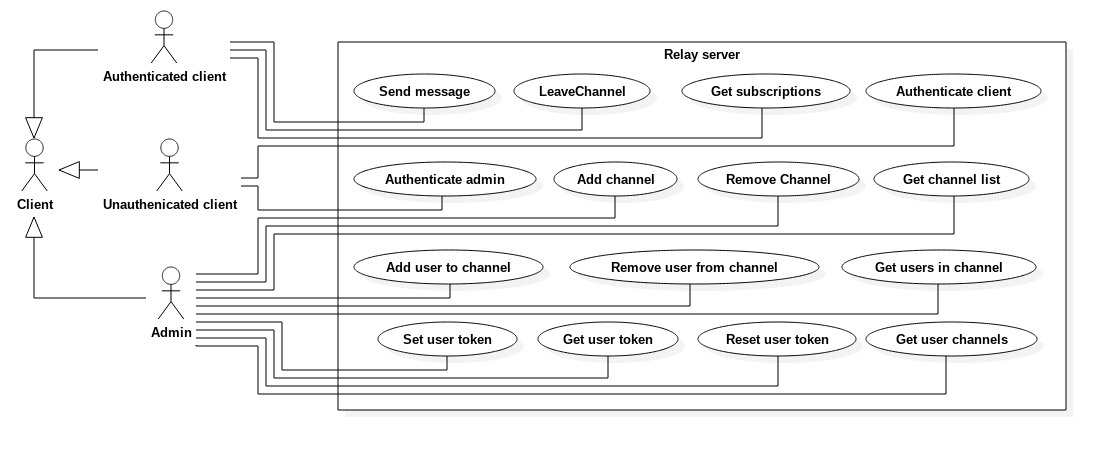
\includegraphics[width=16cm,keepaspectratio]{UML/png/Use Case Model__Use Cases_0}
				\caption{Diagramma usecase}
			\end{center}
		\end{figure}

	 \section{Struttura della piattaforma}
	 \subsection{Diagramma strutturale}
	 Diagramma UML
	 Spiegazione della funzione delle compnenti

	 \subsection{Confronto con soluzioni esistenti}
		\subsubsection{YouTube}
		\subsubsection{Netflix}
		\subsubsection{Red5 Pro}
		\subsubsection{Contus Vplay}
		\subsubsection{Streamroot}
		\subsubsection{Wowza Streaming Engine}

\section{Tecnologie utilizzate}
	\subsection{Linguaggi --- Java}
	 Integrazione facile con Android

	\subsection{Piattaforma --- Tomcat8 EE}

	\subsection{Protocollo --- TCP su WebSocket}

	\subsection{Tipo di dati scambiati --- JSON vs XML}
	 Meno prolisso
	 Scelto per semplificare la codifica della piattaforma
	 Facile a comprendere
	\subsection{Strumetni di supporto}
				\subsubsection{Strumenti di versionamento}
			Git e Bitbucket
				\subsubsection{Strumenti di test e verifica}
			JUnit
				\subsubsection{Strumenti di analisi di rete}
			Wireshark
				\subsubsection{Strumenti di continuous integration}
			Docker
\section{Nuovi orizzonti}
	\subsection{Blockchain}
	\subsection{Streaming peer to peer}

\section{Qualifica}
	\subsection{Verifica}
				\subsubsection{Analisi statica}
				\subsubsection{Analisi dinamica}
	\subsection{Validazione}
				\subsubsection{Validazione interna}
				\subsubsection{Validazione esterna}